\documentclass[a4paper, twocolumn]{article}
\usepackage[a4paper,pdftex]{geometry}
\usepackage[english]{babel}
\usepackage{amsmath,amsfonts}
\usepackage[round]{natbib}
\usepackage[pdftex]{graphicx}
\usepackage{epstopdf}
\usepackage{fancyhdr}
\usepackage{lastpage}
\usepackage{setspace}
\usepackage{xcolor}
\usepackage{hyperref}
\usepackage{url}
\usepackage[all]{xy}
\usepackage[toc,page]{appendix}
\usepackage[T1]{fontenc}
\usepackage{verbatim}
%\usepackage{titling}
\usepackage{multirow}
%\usepackage{multicol}

% Page style.
%\pagestyle{fancy}


% Page header and footer.
%\lhead{}
%\cfoot{}
%\rfoot{\thepage}



\title{Automated Optimization of Walking Parameters for the NAO Humanoid Robot\\
\vspace{.5em}
\begin{center}
	
\includegraphics[scale=.8]{images/uva}\\ \normalsize
	Intelligent Systems Track\vspace{.4em}\\MSc Artifical Intelligence\\Faculty of Science\\ \vspace{.2em}
\end{center}
}
%\posttitle{{}\\\normalsize\textsc{NAO Visual Gait And Trajectory Estimation}\vspace{1cm}}
%\newcommand{\MyuAthors}{
%\small
%\begin{table}[ht]
%\centering
%\begin{tabular}{cccc}
%\multicolumn{4}{c}{Supervisor: Dr. A. Visser}\\\\
%C. Kooijman             &S. Laan               &C. R. Verschoor         &A. J. Wiggers\\
%5743028                 &6036031               &10017321                &6036163\\
%\url{Chiel999@gmail.com}&\url{S.Laan@uva.nl}   &\url{Verschoor@uva.nl}  &\url{A.J.Wiggers@uva.nl}
%\end{tabular}
%\end{table}
%}

\author{
N Girardi\\10457828\\\url{Nickog90@gmail.com} \and
C. Kooijman\\5743028\\\url{Chiel999@gmail.com} \and
A. J. Wiggers\\6036163\\\url{A.J.Wiggers@uva.nl}
}

%%\preauthor{\large\MyAuthors}
%\author{\MyAuthors}
\date{\today}


% OFFICIAL FRONT PAGE
\begin{document}
%\maketitle
%\begin{multicols}{2}
\maketitle
%\clearpage

% TABLE OF CONTENTS
%\thispagestyle{empty}
%\tableofcontents
%\clearpage

\begin{abstract}
	This article describes a framework for optimising walking parameters for a
	NAO bipedal robot, both in a virtual setting and in the real world. It also
	covers preliminary results of the first experiments and provides
	suggestions for future research based on those experiments and the author's
	experience from hand-tuning those parameters.
\end{abstract}

\section{Introduction}
The main focus of the project is improving the walking motion of NAO robots by
optimizing a set of parameters for an existing walking engine. Our research is
specifically about a game competition, the RoboCup Standard Platform League
(SPL), but has also a broader value. Walking is indeed one of the main
challenges in robotics, and robots can be used in many environments to solve
different problems. By walking better robots can move faster and avoid hardware
or environment damages. Walking well allows a robot to reach and function in
places designed for humans. There's an even broader meaning in this work:
To study the effectiveness of different machine learning methods in real
life environments, which means taking into consideration factors such as field
imperfections, sensor error, error in joint angles, and overheating of servos. To work on this
we built a specific framework which would enable us to manage the learning
process and obtain data for evaluation. 

The RoboCup's aim is to promote Robotics and AI research in a playful and
entertaining fashion that would appeal to non-expert people and potential
future generations of researchers \citep{kitano1997robocup}. The event is also
an occasion for insiders to share and expand their knowledge. The competition
factor plays a role by creating an environment which stimulates improvement.
The fact that SPL is mainly about software helps this sharing process, as code
from the winning team has to be published after the end of the competition. 

\begin{figure}
	\center
	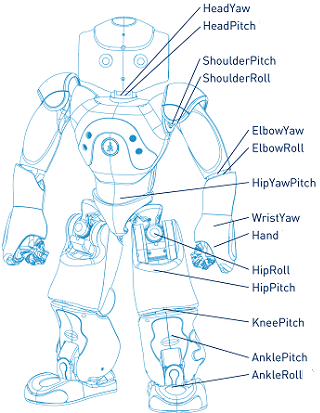
\includegraphics[scale=.85]{images/naospecsJoints}
	\caption{Aldebaran overview of NAO joints.}
	\label{fig:joints}
\end{figure}

\section{Related work}

\subsection{Genetic algorithm}

\citet{macalpineusing} have been successful in the use of a genetic algorithm
to learn to walk on a NAO robot. Their approach uses the CMA-ES policy search,
and did an extensive search of a policy space consisting of 14 out of over 40
parameters.
\citet{meijer2012getting} has applied Finite Difference, Vanilla, Episodic
Natural Actor Critic and a Genetic Algorithm to learn to kick a ball with a
NAO.
A basic genetic algorithm contains at least the following:

\begin{itemize} 
\item Properties that define an organism, the `genes' that can be altered to create new organisms.
\item A population of organisms that is to be evaluated. 
\item A fitness function and corresponding evaluation tasks that specifies how these organisms are evaluated.
\item A way to generate new generations based on old ones. 
\item Learning parameters that influence how new generations are formed. 
\end{itemize}

Through the fitness function and corresponding evaluations, the search can be guided towards a specific direction. A disadvantage of this method is that the fitness function must be user-specified, which may be hard to do in tasks with multiple objectives or in cases where the criteria for performance are unclear. 

The ways in which new generations are generated are similar to biological generation of offspring.  
\begin{itemize} 
\item Transmission of parts of either parent.
\item Crossover between two parents by taking a (weighted) mean of parts of the two.
\item Mutation by adding random elements to the organism.
\end{itemize}


For each generation there is a part of individuals that is copied to the next one. Some of those individuals are picked to generate new individuals using transmission, crossover or mutation. It's important then to set a proper number of survivors and parents in order to have the highest quality features of fittest individuals pass to the next generation without however limiting the search space to a small area. 




\section{Approach}
\subsection{Platform}
The robot which is used in SPL is Nao (version H25) by Aldebaran \citep{gouaillier2009mechatronic}, a humanoid, bipedal robot. It has inertia sensors that enable fall-detection, and a total of eight resistors in the two feet that allow for early detection of inbalance. 

\subsection{Walking engine}
In the RoboCup 2013 we used the NaoTH framework for NAO by Berlin United
\citep{naothdescription} for various reasons: it features a modular code which
makes it easy to expand, and provides a walking engine from which we can select
a set of parameters for learning. 

The walking system is closed loop, and uses a set of more than thirty parameters. A subset of this set was selected manually for learning, as these were likely to contribute to a stable and fast walk than others.
Some examples are:
\begin{description}
\item[singleSupportTime] Defines how long the NAO stands on a foot for during the walking. This determines the walking frequency.
\item[stepHeight] Defines the maximum distance between the ground and the base of the feet. If not too high improves stability, but given the low weight of the robots, if set over a certain limit, makes the robot bounce and actually lose stability. It also requires more work by the joints which translates in overheating and joints' efficiency decreasing. 
\item[maxStep$_{x,y, \theta }$] Defines the maximum length (for walking forward), width (for strafing left and right) and angle (for turning left and right). Given a certain singleSupporTime, those parameters determine the speed of the movements. If set too high the result is a loss in stability.
\item[bodyOffset$_{x}$] The body's offset in $x$-direction (forward). Setting this to a positive number will result in positioning the body forward during walking, which may contribute to faster walking in the $x$-direction.
\item[bodyPitchOffset] Indicates how much the body leans forward during walking with respect to the hips and legs. Similar to bodyOffset in that it can contribute to fast walks in $x$-direction. 
\item[CoMHeight] Height of the center of mass of the robot during walking. The lower the body will be, the more stable the walk. However, the load on the leg joints will be higher and steps must be much smaller than for high center of mass. 
\end{description}

We choose to solve this problem using machine learning methods, as setting and testing these parameters manually is a time-consuming task and does not guarantee selection of an optimal parameter set. The differences between robots (for example actuator and sensor error) cause parameter settings to have a different effect on each robot. Also, the use of machine learning (and, more specifically, reinforcement learning) to learn robots to perform complex tasks is a relevant topic in AI research, and is a problem that is not limited to NAO robots, but applies to many other situations. 


\section{Implementation}
The NaoTH framework is a modular framework that runs iteratively.  For the use of machine learning methods described in the previous section, it was extended by a module `MachineLearning', which serves as a generic input for different machine learning methods. It consists of multiple classes:
\begin{description}
\item[MachineLearning] The module class itself, handles debug requests from users.
\item[LearnToWalk] The evaluation program, used by the module to test performance of specific parametersets.
\item[MachineLearningMethod] An abstract class that contains pure virtual functions, to be implemented by classes corresponding to specific machine learning methods.
\end{description}

This module can be controlled through debug requests. Alongside the module, an interface was created for easy parameter selection and the display of information during learning.

\subsection{Learning Parameters}

To manage and control the genetic algorithm we implemented a GUI from which we can set specific parameters:

\begin{description}
\item[crossoverRate] Defines the weight for crossover.
\item[mutationRate] Defines the weight for mutation.
\item[trasmitRate] Defines the weight for transmission.
\item[maxGeneration] The maximum number of generations that can be evaluated before the learning process ends. 

\item[parentsNum] The number of individuals from a generation that are used to obtain a new generation.
\item[populationSize] The number of individuals for each generation.
\item[resettingTime] Time before the NAO touches the ground after a previous evaluation has ended.
\item[runningTime] Duration of an evaluation.
\item[standingTime] Time during the NAO stays still after touching the ground before starting a new evaluation. It's used to guarantee stability for the body when starting an evaluation.
\item[surviveNum] The number of individuals that are copied from a generation to the next one. 

\end{description}

\subsection{Evaluation Tasks}

The evaluation tasks that were defined to run the tests are:

\begin{itemize}
\item Walk forward/backward 
\item Strafe left/right 
\item Turn right/left x degrees 
\item Walk diagonally (walk forward/backward + strafe left/right) 

\end{itemize}

Those tasks can be combined to obtain more realistic and challenging action sequences.
% TODO pic interface + screen

\subsection{Fitness Function}

The walking distance is at the base of the fitness function used in the 
experiments. To emphasise that the robot should be able to walk in any 
direction, each evaluation consists of a set of tests, which can include
walking forward, backward, sideways (strafing), rotating, and walking
diagonally in any direction, we use the weighted harmonic mean (equation
\ref{eq:harmonic}).

\begin{equation}
    \frac{∑ⁿᵢ=₁ wᵢ} {∑ⁿᵢ=₁\frac{wᵢ}{xᵢ}}
    \label{eq:harmonic}
\end{equation}
The weights allow for focusing more on specific tasks such as walking forwards.
The framework allows for giving a negative reward when the robot falls over.
The individual can be killed to save time and reduce the chance of damage in
the case of testing in the real world.

\section{Results}

\subsection{Experiments}
The graph in figure \ref{fig:avg} shows how the average fitness of the population changes over time. The shown results are promising, as the fitness is generally growing in the first 25 generations. 

The graph in figure \ref{fig:max} shows the fitness of the fittest individual in the population over time, which is monotonically increasing. That's because the surviving group of each population, of which the fittest individual is part of, is not re-evaluated. 

\subsection{Results in RoboCup 2013}
Using the walking parameters that were result of a partial learning process using both simulation and real life environment, there has been a visible improvement in performance of our team of robots, compared to the previous competition (Iran Open 2013  \footnote{http://2013.iranopen.ir/}). 

\begin{figure}
	\center
	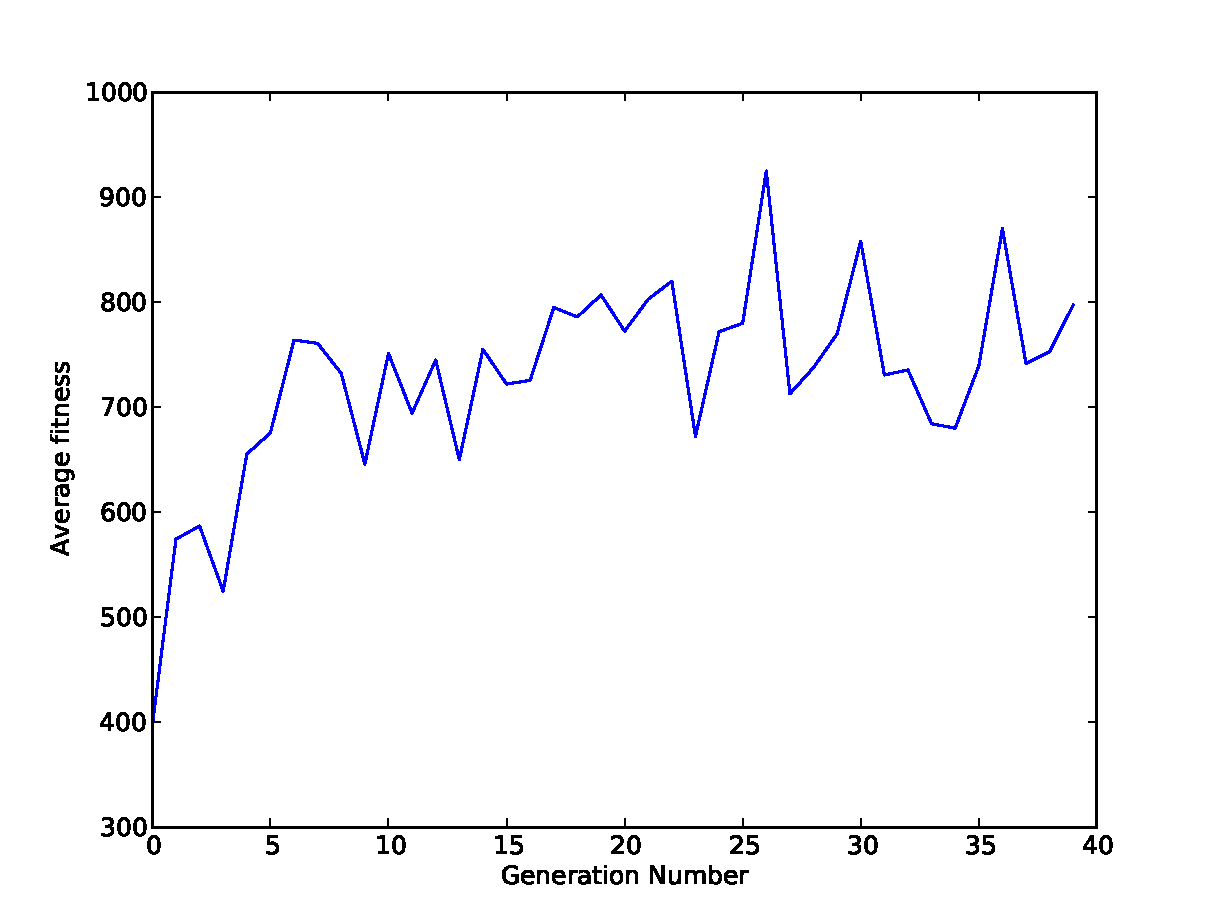
\includegraphics[width=.5\textwidth]{images/fitness}
	\caption{Average fitness of the population over time.}
	\label{fig:avg}
\end{figure}

\begin{figure}
	\center
	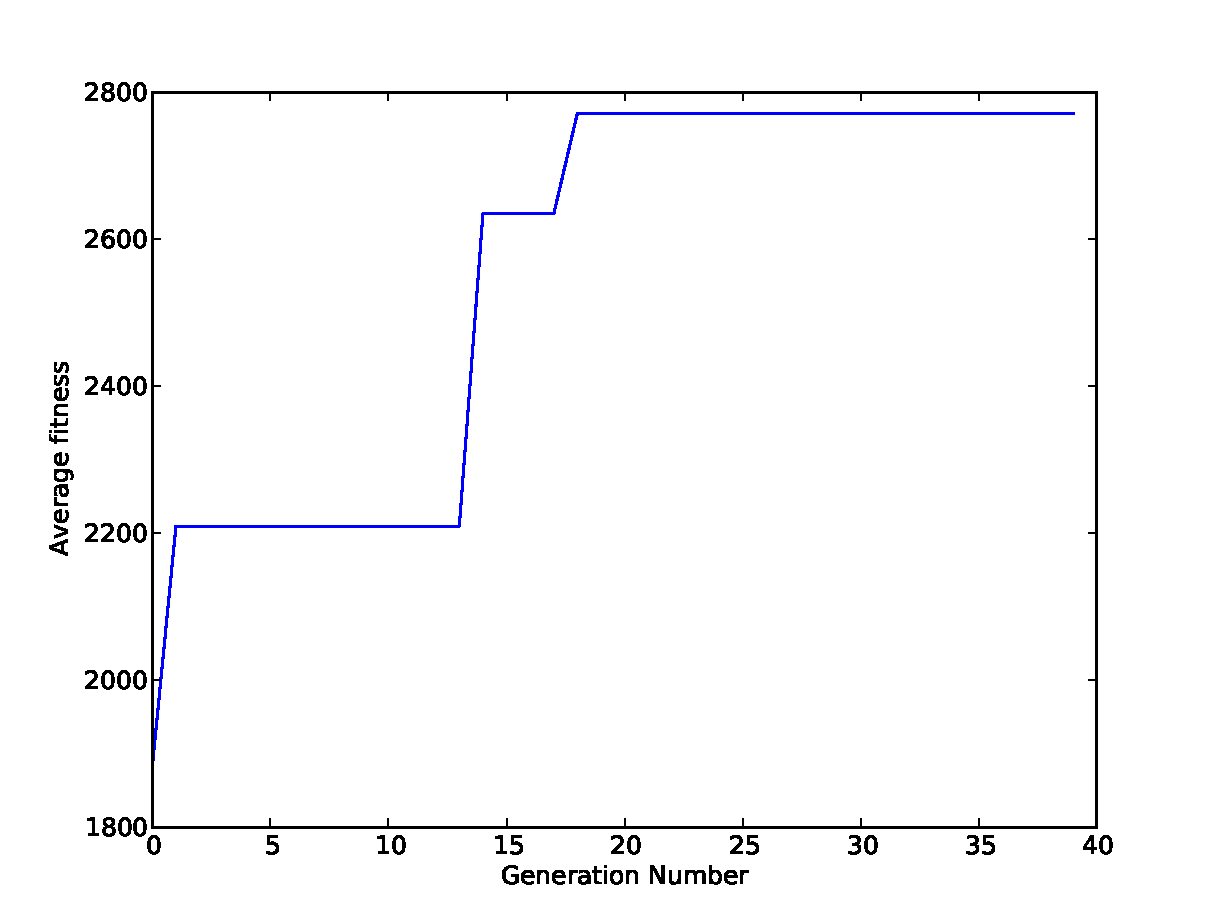
\includegraphics[width=.5\textwidth]{images/max_fitness}
	\caption{Maximum fitness of the population over time.}
	\label{fig:max}
\end{figure}


 

\section{Future Work}
 

In the future we look forward to working on online learning, that is learning during matches, for several reasons. First, there are some conditions and situations that are difficult to recreate in lab or in simulation. Also the learning process is time consuming and by using online learning we can exploit matches as an opportunity to have more time to improve our results. To do that it's necessary to classify different kind of actions sequences in order to learn different sets of parameters for each of them. Also we need to find a way to predict what kind of sequence of actions is about to be performed in order to chose what set of parameters to apply during a match. We think this would give a big improvement to our game as different actions ,such as walking forward or turning, work better with different settings. It would be easy to implement different parameters for each action, but that wouldn't make such a difference as working on different sets of actions. That's because actions such as staying still don't require any particular parameter set per se, but if combined with other actions such as walking forward (so, for example, doing a few steps and stop) specific values are needed for the parameters. 


\bibliographystyle{plainnat}
\bibliography{references}
\end{document}

